\item In Figure 1, $O$ is the centre of a circle, $PQ$ is a chord, and $PT$ is the tangent at $P$. If $\angle{POQ}$=$70\degree$, then $\angle{TPQ}$ equal to
    \begin{figure}[H]
    \centering
    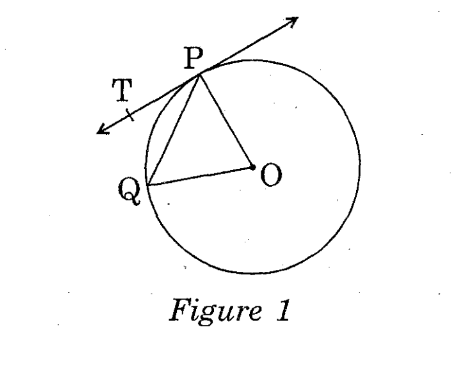
\includegraphics[width=0.8\columnwidth]{figs/figure1.jpg.png}
    \end{figure}
    \begin{enumerate}[label=(\Alph*)]
        \item $55\degree$
        \item $70\degree$
        \item $45\degree$
        \item $35\degree$
    \end{enumerate}
    
    \item In Figure $2$, $AB$ and $AC$ are tangents to the circle with center $O$ such that $\angle{BAC} = 40\degree$. Then $\angle{BOC}$ is equal to
    \begin{figure}[H]
    \centering
    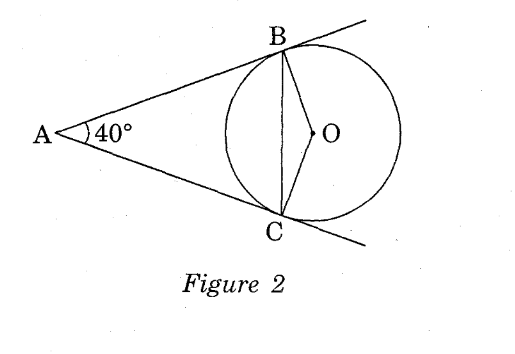
\includegraphics[width=0.8\columnwidth]{figs/figure2.jpg.png}
    \end{figure}
    \begin{enumerate}[label=(\Alph*)]
        \item $40\degree$
        \item $50\degree$
        \item $140\degree$
        \item $150\degree$
    \end{enumerate}

    \item Draw a pair of tangents to a circle of radius $3$ cm, which are inclined to each other at an angle of 60\degree.


    \item In Figure $3$, a circle touches all the four sides of whose sides are $XB = 6$ cm, $BC = 9$ cm, and $CD = 8$ cm. Find the length of side $AD$.
 \begin{figure}[H]
    \centering
    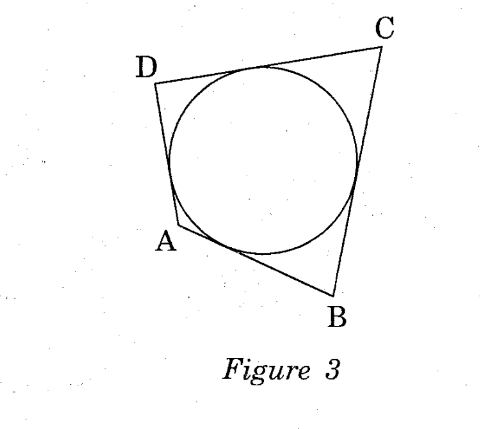
\includegraphics[width=0.8\columnwidth]{figs/figure3.jpg.png}
 \end{figure}
 
 \item Prove that the tangent at any point of a circle is perpendicular to the radius through the point of contact.
 
  

  \item A chord of a circle of radius $14$ cm subtends an angle of $120\degree $ at the center. Find the area of the corresponding minor segment of the circle. 

[Use $\pi = \dfrac{22}{7} = x$ and $\sqrt{3} = 1.73$]
\item In Figure $6$, three circles each of radius $3.5$ cm are drawn in such a way that each of them touches the other two. Find the area enclosed between these three circles (shaded region).

[Use $\pi = \dfrac{22}{7}$]
 \begin{figure}[H]
    \centering
    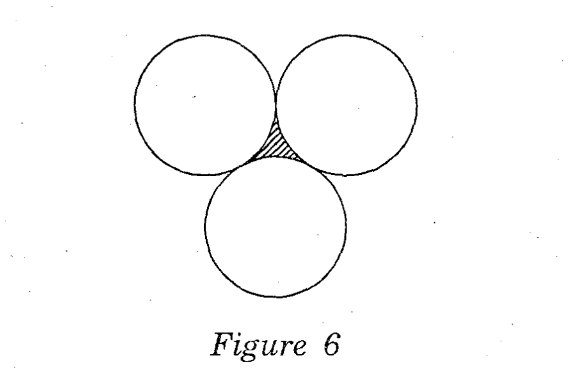
\includegraphics[width=0.8\columnwidth]{figs/figure6.jpg.png}
 \end{figure}

 \item  Find the perimeter of the shaded region in Figure $4$, if $ABCD$ is a square of side $14$ cm and $APB$ and $CPD$ are semicircles. [Use $\pi = \dfrac{22}{7}$]
\begin{figure}[H]
    \centering
    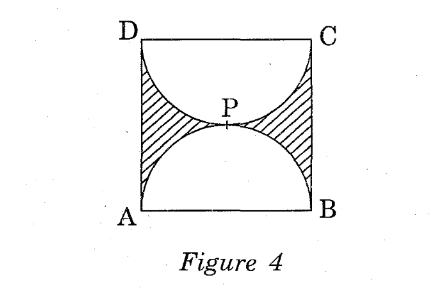
\includegraphics[width=0.8\columnwidth]{figs/figure4.jpg.png}
 \end{figure}

 \item  In Figure $5$, a triangle $PQR$ is drawn to circumscribe a circle of radius $6$ cm such that the segments $QT$ and $TR$ into which $QR$ is divided by the point of contact $T$, are of lengths $12$ cm and $9$ cm respectively. If $[PR]$, the area of $PQR$, is $40\, \text{cm}^2$, then find the lengths of sides $PQ$ and $PR$.
\begin{figure}[H]
    \centering
    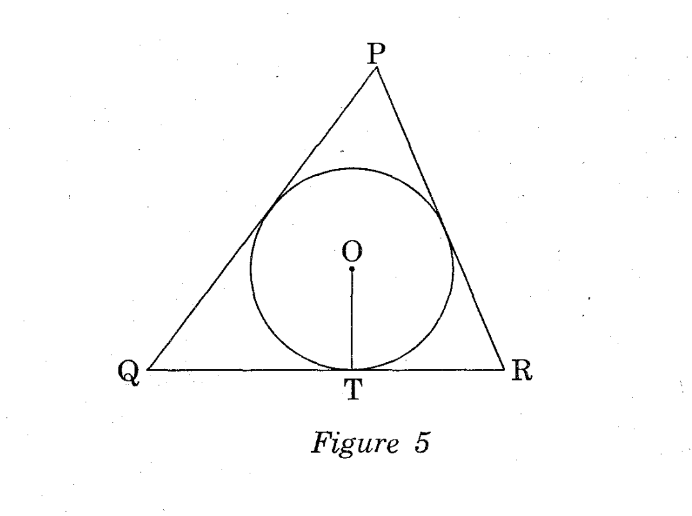
\includegraphics[width=0.8\columnwidth]{figs/figure5.jpg.png}
 \end{figure}
\end{enumerate}
